@@ -1,465 +0,0 @@
\section{Tables}\label{Appendix:Tables}
\section{Code Snippets}\label{Appendix:CodeSnippets}
{
\begin{lstlisting}[language=XML]
//Sample code of a rotating Bezier spline that will render the Urdu letter Aa'en in Nastaleeq.
<spline>
    <FlatTipWidth>150</FlatTipWidth>
    <Color>-5658199</Color>
    <anchor>
      <rotationoffset>0</rotationoffset>
      <P>-198.3791, 452.6993</P>
      <C1>-131.6351, 572.4461</C1>
      <C2>-265.1234, 332.9534</C2>
      <R1>-148.3791, 452.6993</R1>
    </anchor>
    <anchor>
      <rotationoffset>0</rotationoffset>
      <P>-296.5323, 156.2775</P>
      <C1>-439.8357, 254.4304</C1>
      <C2>-119.5302, 35.04326</C2>
      <R1>-246.5322, 156.2775</R1>
    </anchor>
    <anchor>
      <rotationoffset>0</rotationoffset>
      <P>25.40986, 374.1774</P>
      <C1>-47.22344, 262.2825</C1>
      <C2>98.04301, 486.0714</C2>
      <R1>75.40986, 374.1774</R1>
    </anchor>
    <anchor>
      <rotationoffset>0</rotationoffset>
      <P>-233.7143, -183.332</P>
      <C1>-208.1945, -28.25013</C1>
      <C2>-274.7982, -432.9961</C2>
      <R1>-183.7143, -183.332</R1>
    </anchor>
    <anchor>
      <rotationoffset>0</rotationoffset>
      <P>315.9428, -517.0526</P>
      <C1>95.77186, -679.5702</C1>
      <C2>435.6645, -428.6809</C2>
      <R1>365.9427, -517.0526</R1>
    </anchor>
    <anchor>
      <rotationoffset>0</rotationoffset>
      <P>441.5787, -144.0708</P>
      <C1>388.576, -277.5591</C1>
      <C2>494.5813, -10.58265</C2>
      <R1>491.5787, -144.0708</R1>
    </anchor>
  </spline>
\end{lstlisting}
}
\section{Images}
{

\begin{figure}[H]
  \centering
  \includegraphics[width=0.8\textwidth]{../Images/Nastaleeq_Ink.pdf}
  \caption
  {
      Nastaleeq sample by Gohar Qalam. (a) Original calligraphy photo. (b) Original photo processed for analysis. (c) Traced rotating bezier spline ink. (d) Difference between (b) and (c). The red pixel indicate the portions that are missing in (c) but are present in (b) and the blue ones show the missing pixels in (b) but are present in (c).
  }
\end{figure}

\begin{figure}[H]
  \centering
  
\includegraphics[width=0.8\textwidth]{../Images/Nastaleeq_Machined.pdf}
  \caption
  {
      Machined Nastaleeq sample by Gohar Qalam. (a) Rasterized rotating bezier spline for machining (b) Ink marks machined by a simulated robotic manipulator. (c) and (d) are differences between simulated ink mark and the rasterized photo and the processed original photo respectively. The red pixel indicate the portions that are missing in (c) but are present in the reference image and the blue ones show the missing pixels in reference but are present in the ink mark.
  }
\end{figure}

\begin{figure}[H]
  \centering
  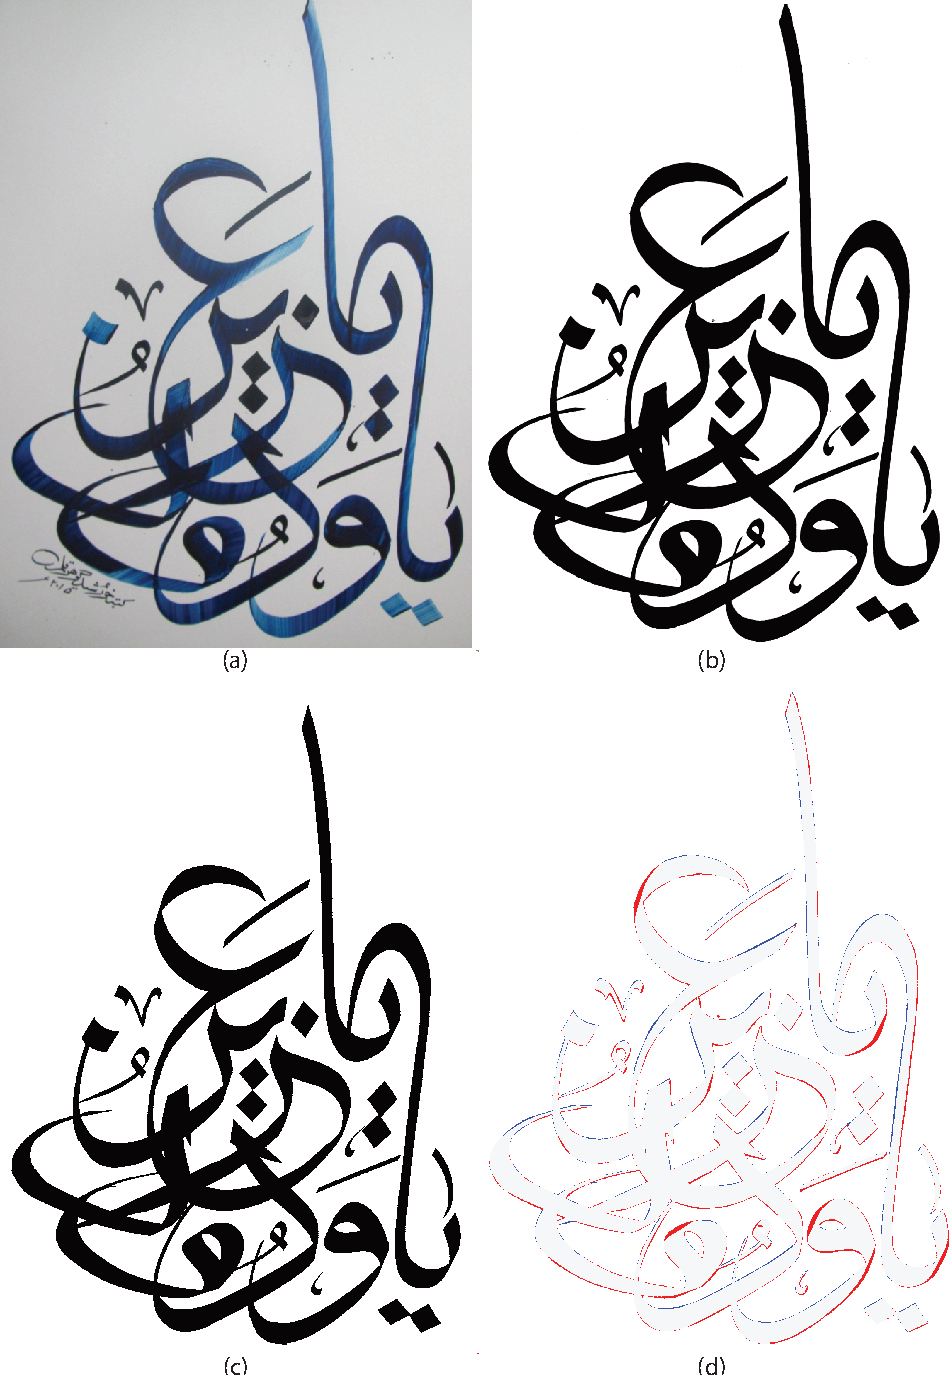
\includegraphics[width=0.8\textwidth]{../Images/Thuluth_Ink.pdf}
  \caption
  {
      Thuluth sample by Gohar Qalam. (a) Original calligraphy photo. (b) Original photo processed for analysis. (c) Traced rotating bezier spline ink. (d) Difference between (b) and (c). The red pixel indicate the portions that are missing in (c) but are present in (b) and the blue ones show the missing pixels in (b) but are present in (c).
  }
\end{figure}

\begin{figure}[H]
  \centering
  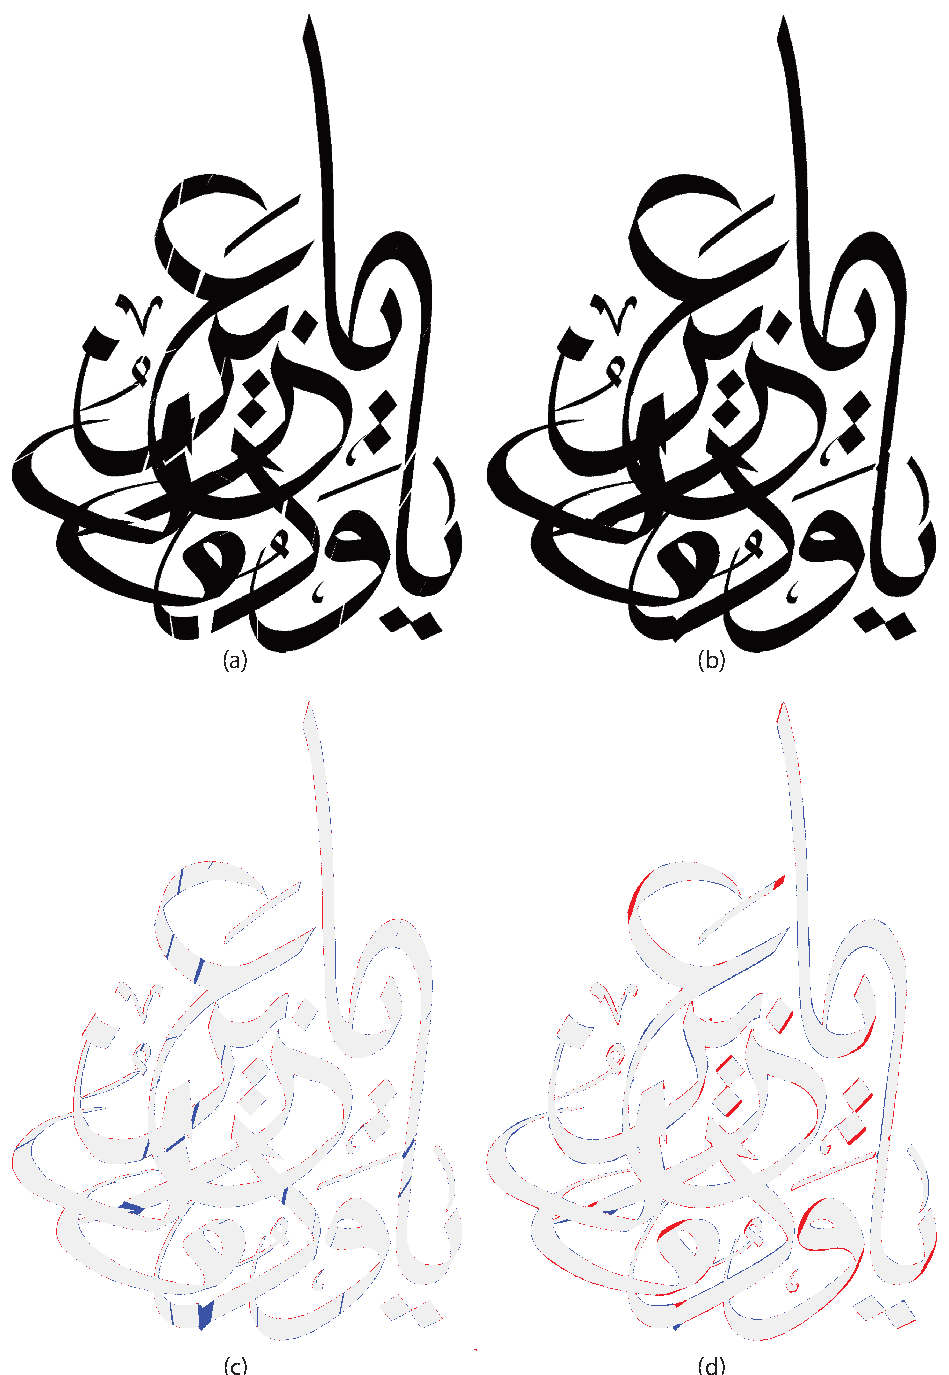
\includegraphics[width=0.8\textwidth]{../Images/Thuluth_Machined.pdf}
  \caption
  {
      Machined Thuluth sample by Gohar Qalam. (a) Rasterized rotating bezier spline for machining (b) Ink marks machined by a simulated robotic manipulator. (c) and (d) are differences between simulated ink mark and the rasterized photo and the processed original photo respectively. The red pixel indicate the portions that are missing in (c) but are present in the reference image and the blue ones show the missing pixels in reference but are present in the ink mark.
  }
\end{figure}
} 